
% figure balanced parentheses binary trees
% add figures/exhaustive lists
\section{Combinatorial Generation: Looking at All the Possibilities}

Combinatorial generation is defined as the exhaustive listing of combinatorial objects of various types.  Frank Ruskey duly notes in his book \emph{Combinatorial Generation} that the phrase ``Let's look at all the possibilities" sums up the outlook of his book and the field as a whole \cite{ruskey2003combinatorial}. Examining all possibilities fitting certain criteria is frequently necessary in fields ranging from mathematics to chemistry to operations research. Combinatorial generation as an area of study seeks to find an underlying combinatorial structure to these possibilities and utilize it to obtain an algorithm to efficiently enumerate an appropriate representation of them \cite{ruskey2003combinatorial}. 

Combinatorial generation is a field of study that has many parallels to sorting.  Like sorting, it is a fundamental computational task that will be run on computers for decades.  Additionaly, in the same way that different sorting algorithms work better for different types of data, different combinatorial generation algorithms may be better suited for different types of tasks.  This makes combinatorial generation an important area of study for making many common tasks more efficient.  

Unlike sorting, however, combinatorial generation is not widely taught and is rarely discussed in core textbooks. Notable exceptions to this are volume 4A of The Art of Computer Programming by Don Knuth \cite{knuth2015art}, initially published in 2011, and Kreher and Stinson's textbook \emph{Combinatorial Algorithms: Generation, Enumeration, and Search} \cite{kreher2020combinatorial}.

\subsection{Lexicographic Orders}
Lexicographic order is the simplest and most intuitive way of enumerating combinatorial objects.  Moreover, enumerating a set of combinatorial objects in lexicographic order is always possible. Any combinatorial object handled by computers must be encoded in binary somehow; therefore any combinatorial object can be enumerated in lexicographic order via the lexicographic order of its binary representations. 

TODO: different ways to implement lex (i.e., scan for location of change, or keep track and predict) ? 

In addition to traditional lexicographic order, there are a couple of simple variations on it. Co-lexicographic order generates object as if they were being generated via a lexicographic ordering of strings with the most significant bit at the right end of the string instead of the left.  Where lexicographic order increments the rightmost bit and carries to the left, co-lexicographic order increments the leftmost bit and carries to the left. Reverse lexicographic order generates objects in the reverse order of lexicographic: it order objects from lexicographically largest to lexicographically smallest. Co-lexicographical order can also be reversed in this way to generate reverse co-lexicographic order. Figure \ref{fig:bintable} demonstrates lexicographic, co-lexicographic, and reverse lexicographic order for binary strings with $n$ bits.

Continuing with the comparison of combinatorial generation to sorting, lexicographic and co-lexicographic orders are much like insertion and selection sort.  They are fairly intuitive, easy to implement, and sometimes ``good enough."  However, they are rarely optimal: more thoughtful orderings will frequently have significant performance advantages over lexicographic orderings. In particular, lexicographic orderings often require worst-case $O(n)$ time per generated object, whereas \emph{loopless} generation algorithms that use only worst-case constant time per generated object are often achievable. The term loopless refers to the fact that, typically, a worst-case $O(1)$ algorithm can be implemented without any inner loops.

\begin{figure}[]

\begin{center}
\begin{tabular}{ |c|c|c|c|c| } 
 \hline


n &  lex  & colex & revlex & Gray \\  
\hline
0 & 0000 & 0000 & 1111 & 0000 \\
1 & 0001 & 1000 & 1110 & 0001 \\
2 & 0010 & 0100 & 1101 & 0011 \\
3 & 0011 & 1100 & 1100 & 0010 \\
4 & 0100 & 0010 & 1011 & 0110 \\
5 & 0101 & 1010 & 1010 & 0111 \\
6 & 0110 & 0110 & 1001 & 0101 \\
7 & 0111 & 1110 & 1000 & 0100 \\
8 & 1000 & 0001 & 0111 & 1100 \\
9 & 1001 & 1001 & 0110 & 1101 \\
10 & 1010 & 0101 & 0101 & 1111 \\
11 & 1011 & 1101 & 0100 & 1110 \\
12 & 1100 & 0011 & 0011 & 1010 \\
13 & 1101 & 1011 & 0010 & 1011 \\
14 & 1110 & 0111 & 0001 & 1001 \\
15 & 1111 & 1111 & 0000 & 1000 \\

\hline

\end{tabular}

    (too early for Gray code here?)
\end{center}
        \caption{The $2^5$ $5$-bit binary strings generated lexicographic, co-lexicographic, reverse lexicographic, and Gray code order.}
        \label{fig:bintable}
\end{figure}


\subsection{Binary Reflected Gray Code}

A quintessential result of the combinatorial generation in practice is Frank Gray's reflected binary code, or Gray code. Gray codes give a ``reflected" ordering of binary strings such that each successive string in the ordering differs from the previous string by exactly one bit. This contrasts from a lexicographic ordering of binary strings, in which a n-digit binary string can differ by up to n digits from its predecessor and will differ by approximately two (more precisely $\sum_{i=0}^n2^i$, which is 1.9375 for 4 bit values and 1.996 for 8 bit values) bits on average\footnote{Consecutive pairs of binary digits in lexicographic order will differ in the bit at position i with probability $\frac{1}{2^i}$.  Therefore, the average number of differing bits between two binary strings of length n is $\sum_{i=0}^n2^i$, which converges to 2 as n grows large.}. The binary reflected Gray code, therefore, provides an ordering that requires half as many bit switches on average as the more intuitive lexicographic order. 



Binary reflected Gray codes are especially useful in electromechanical switches to reduce physical error and prevent spurious output associated with asynchronous bit switches.  In particular, changing multiple bits per iteration can result in ``in-between" states where some but not all of the bit changes necessary for a switch have been executed.  One can think of this like an odometer on a car: When changing from $99999$ to $100000$ miles, the odometer might briefly read $000000$, or $19999$, or $10009$, or any number of other ``in-between" states. 

This issue can occur in cases as simple as incrementing $3$ to $4$.  In lexicographic order, the string must change from $011$ to $100$ in lexicographic order; in Gray code order it changes from $010$ to $110$.  The lexicographic change requires three bit changes; the Gray code order requires only one.  When using physical switches, three bit changes are unlikely to change in exact synchrony.  This creates the possibility of reading $101$, $110$, $111$, or \emph{any other 3-bit binary number} if the switches are read mid-change, depending on the order of the bit changes.  When using the binary reflected Gray code, the only states are $3=010$, the previous value, and $4=110$, the correct next value. One could easily imagine a test, such as checking if a number is less than $5$, that could evaluate incorrectly due to reading during the change between $3=011$ and $4=100$ in lexicographic order.  This type of error is eliminated by using a Gray code ordering that changes only one bit per iteration.

The approach of ``reflecting'' sublists employed by the binary reflected Gray code is one of the most widely used approaches in combinatorial generation. TODO: explain, give examples, cite \ref{sawada2021inside}.

Frank Gray's binary reflected code was influential enough that the term \emph{Gray code} is often used as a general term for any minimal change ordering of combinatorial objects.  If lexicographic orderings with worst-case $O(n)$ time per generated object are like $O(n^2)$ sorting algorithms, Gray codes are analogous to more efficient sorting algorithms like merge sort, quick sort\footnote{Quicksort is actually worst-case $O(n^2)$, but has better average performance than simple $O(n \log(n))$ sorting algorithms like mergesort or heapsort.  This is due to space efficiency and cache performance, among other things.  Other sorting algorithms like introsort, pdqsort, and Timsort use hybrid approaches to obtain quicksort-like (or better) average performance while maintaining $O(n \log(n))$ worst-case runtime.}, or radix sort.  Gray codes perform iterations by modifying a single object in place, not generating a new object from scratch.  This is almost a hard requirement for achieving better than $O(n)$ time per object, as generating an object of size $n$ from scratch is always at least $O(n)$.



\begin{figure}
    \centering

\includegraphics[width=4in]{BLX6-cropped.pdf} 

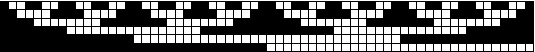
\includegraphics[width=4in]{BRGC6-cropped.pdf} 


\includegraphics[width=4in]{BCLX6-cropped.pdf} 

    \caption{Lexicographic (top), binary reflected Gray code (middle), and cool-lex (bottom) enumerations of 6-bit binary strings. \\ 
    Individual strings are read vertically with the most significant bit at the top; white is 1.
    }
    \label{binary}
\end{figure}

\section{Gray Codes for Trees and Strings} \label{sec:intro_Graycodes}

This thesis aims to create efficient minimal change orderings for other objects: namely, ordered trees and Lukasiewicz words.  Ordered trees and Lukasiewicz words are both \emph{Catalan Objects}.  The number of Lukasiewicz words of length $n+1$ and the number of ordered trees with $n+1$ nodes are both counted by the $n\thh$ Catalan number $\C_n$.  

Frank Gray's reflected binary code used complementing a single bit as the minimal change between successive binary strings in its ordering.  Other notions of minimal changes in strings are \emph{adjacent-transpositions}, or \emph{swaps}, which interchange two adjacent symbols in a string, and \emph{shifts}, in which a single symbol in a string moved to another position. Lukasiewicz words are typically represented as strings of integers, and therefore can make use of these minimal change string operations.  Our Gray codes for Lukasiewicz words will use a slightly more restrictive type of shift, a \emph{left-shift}, which moves a single symbol somewhere to the left within a string. 




% WHAT DOES IT MEAN TO HAVE A MINIMAL CHANGE ORDERING IN A TREE?

% PICTURE? ESA IMAGE? BUT WITHOUT STACK?

% MOVE LSHIFT DEF TO SEC 3?
% NOT JUST OF THEORETICAL INTEREsT, VERY EFFICIENT


Defining minimal changes for trees is more complicated, as what changes are \emph{minimal} within a tree is often representation dependent.  Our Gray code for ordered trees aims to use simple operations that are minimal for most reasonable tree representations.  These minimal changes ``pops", which remove a node's first child, and ``pushes,'' which push one node to be the first child of another.  More specifically, the algorithm will generate trees using a pop-push operation that pops one node's first child and pushes it to become the first child of another node.  We will refer to this pop-push operation as a ``pull.''

TODO: picture

\section{Cool-Lex Order}

HAS BENEFITS OF LEX AND GRAY CODE
% connect Gray code and cool-lex order
Cool-lex order has introduced the idea of rotating sublists to enumerate languages.  Different versions of cool-lex order have been shown to enumerate several sets of combinatorial objects, including binary strings, fixed weight binary strings, Dyck words, and multiset permutations \cite{williams2009shift}.  Cool-lex orders often lead to algorithms that are faster and simpler than standard lexicographic order, and as such are not just of theoretical interest.  For example, the ``multicool" package in R uses a loopless cool-lex algorithm to efficiently enumerate multiset permutations.   The package started using cool-lex order for multiset permutations in version 1.1 and as of version 1.12 has been downloaded nearly a million times \cite{multicool_2021}.  Additionally, Don Knuth included the cool-lex algorithm for Dyck words in his 4th volume of \emph{The Art of Computer Programming} and provided an implementation of it for his theoretical MMIX processor architecture due to its efficiency and simplicity \cite{knuth2015art}.
Two common threads in the cool-lex algorithms for combinatorial generation is their focus on the \emph{non-increasing prefix} of string and their use of \emph{left-shifts} (TODO:is this accurate? should it just be shifts, not left shifts specifically?) for minimal changes.  Mentioned previously in section \ref{sec:intro_Graycodes}, a left shift can be defined formally as follows:

If $\alpha = a_1 a_2 \ldots a_n$ is a string and $i < j$, then we let
\begin{equation}
    \lshiftindex[\alpha]{i}{j} = a_1 a_2 \ldots a_{i-1} a_j a_{i} a_{i+1} \ldots a_{j-1} a_{j+1} a_{j+2} \ldots a_n. \label{eq:leftdef}
\end{equation}

$\lshiftindex[\alpha]{i}{j}$ can also be thought of as rotating the $i$ through $j\thh$ symbols of $\alpha$ right circularly by one.


\section{Goals of this Thesis}

% Cool-lex order has been shown to provide a minimal change cyclic ordering for Dyck words and binary trees. This thesis provides a new algorithm fo

This thesis has the broad goal of extending cool-lex order to new objects.

This thesis will provide two primary contributions, each with sub-contributions.  

The first contribution is a `pop-push' Gray code for enumerating ordered trees in $O(1)$ time. Chapter \ref{chap:otree-graycode} will give a two-case successor rule for generating all ordered trees with $n$ nodes using at most two ``pull'' operations. Chapter \ref{chap:otree-implementation} will provide a loopless algorithm for the successor rule in \ref{chap:otree-graycode} and an implementation of the algorithm in C.

The second contribution is a shift Gray code for Lukasiewicz words.  Chapter \ref{chap:luka-graycode} will give a shift Gray code for generating Lukasiewicz words with fixed content using one prefix shift per iteration.  Chapter \ref{chap:luka-implementation} will give a loopless implementation of the algorithm in \ref{chap:luka-graycode} using an array based implementation for the special case of Motzkin words and a linked list implementation for the general case of unrestricted Lukasiewicz words.

TODO: cite iwoca, esa
